% Threat model and methods (Task 42): old Methods and the constraint part of the old Setup, with A8x, A6x, the
% Stage B control attackers and the outcome rules added. Every result number is a macro (paper_v3/generated/numbers.tex).
\section{Threat Model and Methods}
\label{sec:methods}

Figure~\ref{f_pipeline} gives an overview.

During the preparation of this work the authors used Claude Opus 5.5 (Anthropic), through Claude Code, in order to write
and debug the analysis code and to draft and edit the manuscript text under the direction of the first author, and
Claude Sonnet 5.5 (Anthropic), used by the first author through the Claude app in a separate session, in order to review
intermediate results and to draft the instructions given to Claude Code.
After using these tools, the authors reviewed and edited the content as needed and take full responsibility for the
content of the published article.
The authors also checked the numerical results with scripts, and the first author checked them manually against the
result files.
The analysis code added in this version (the adaptive attacks on the control detectors, the attackers A8x and A6x
and their summaries) was also written by Claude Opus 5.5 through Claude Code under the direction of the first author.

Every number in the paper is generated from the result files by scripts and inserted as a macro, and the authors checked the numbers against the result files.

\begin{figure*}[t]
  \centering
  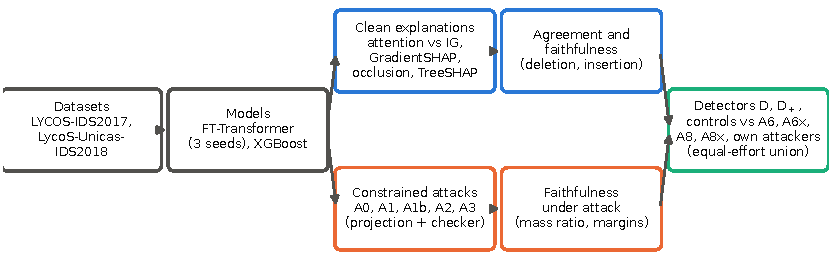
\includegraphics[width=\textwidth]{f_pipeline}
  \caption{Pipeline of the study.}
  \label{f_pipeline}
\end{figure*}

\subsection{Threat model}
\label{sec:threat}
The defender runs a flow classifier, an FT-Transformer, and a learned attack detector on top of it.
The attacker holds a malicious flow and wants the classifier to predict it as benign while the detector stays below its
threshold.
The attacker knows the weights of the classifier and of the detector (white box) and can change only the flow features
that a sender controls, within a per-feature budget and under the protocol relations of the constraint model below.
We consider three levels of attacker knowledge about the detector: none (the attacker ignores the detector), a
differentiable approximation of its scores (stand-ins), and its exact score, with surrogate gradients only where the
exact gradient is zero almost everywhere.
Following the adaptive-attack principle \cite{tramer2020,carlini2017}, a detector is judged by the attacker that models
it, and two detectors are compared at equal attacker effort.
Packet-level attacks, black-box attackers and attacks on the training data are out of scope.

\subsection{Constraint model and validity checker}
\label{sec:constraints}
Of the \nFeatures{} features, \nControls{} are controls the attacker may change within a budget, \nDerived{} are
derived and recomputed from the controls, and \nImmutable{} are immutable (Table~\ref{t_constraints}).
The budget of a control is $\epsilon$ times its clean value, or $\epsilon$ times the training median of its non-zero
values when the clean value is zero.
Class families whose mechanism is the timing and packet count (slow DoS, port scan) have those controls frozen.
A separate validity checker, written as NumPy code apart from the derivation and projection that the attacks use,
re-derived every relation from the written specification and accepted every constrained adversarial row of every
reported attack and detector experiment (Table~\ref{t_constraints}; for the adaptive attacks added in this version,
\sbInvalid{} invalid of \sbRows{} rows on the controls, \axInvalid{} of \axRows{} for A8x and \sxInvalid{} of
\sxRowsWritten{} for A6x).
It shares the specification file and a few helpers with the attack code, so it shows internal consistency rather than
realisability.

% Generated by paper/make_tables_v2.py on 2026-10-30. Do not edit.
% Source: results/stage4_constraints.csv
% Source: results/stage7/stage7d/stage7d_frozen_share.csv
% Source: results/stage7/stage7d/stage7d_frozen_share_2017.csv
\begin{table}[t]
\centering
\footnotesize
\caption{Constraint model of the constrained attacks.}
\label{t_constraints}
\begin{tabular}{lc}
\toprule
Feature role & Count \\
\midrule
Features in the model & $72$ \\
Controls (attacker-perturbed, budgeted) & $18$ \\
\quad of which add-only & $9$ \\
\quad of which either direction & $9$ \\
\quad of which integer & $15$ \\
Derived (recomputed from controls) & $16$ \\
Immutable & $38$ \\
\midrule
\multicolumn{2}{l}{\textit{Class-family freezes (controls frozen because they are the attack mechanism)}} \\
slow dos (2017: DoS Slowhttptest, DoS Slowloris; 2018: DoS Slowloris) & $10$ \\
scan (2017: PortScan; 2018: none) & $10$ \\
\bottomrule
\end{tabular}
\par\smallskip\parbox{\linewidth}{\scriptsize Budget per control and row: $\epsilon$ times the clean value, or $\epsilon$ times the training median of the non-zero values when the clean value is 0 (training split of each dataset). A separate checker validates every adversarial row: 0 invalid of 336{,}093 saved constrained adversarial row records (both datasets, all reported attack and defender experiments; the defender experiments reuse the A1 rows of the attack experiments).}
\end{table}


\subsection{Explanations and faithfulness}
For each FT-Transformer we computed three attention variants over the \nFeatures{} feature tokens: the [CLS] row of the
last layer averaged over heads, the [CLS] row averaged over layers and heads, and attention rollout
\cite{abnar2020}.
A single attention head selected on validation data served as a diagnostic (Appendix~\ref{sec:appendix}).
As references we used IG with the training mean as baseline, GradientSHAP, leave-one-feature-out occlusion, TreeSHAP of
an XGBoost model, the absolute standardised input $|x|$, and a random ranking.
Signed attributions were ranked by their absolute value.

Agreement between two explanations is the Spearman correlation of their feature rankings per row.
Faithfulness was measured by masking features in ranking order with the training mean and recording the probability of
the explained class: the area under the deletion curve (lower is more faithful) and under the insertion curve (higher
is more faithful) \cite{petsiuk2018,samek2017}.
On adversarial rows we used the logit margin of the original class and the gap between most- and least-relevant-first
removal (AOPC gap, where AOPC is the area over the perturbation curve) \cite{samek2017}, and subtracted the change measured under the random control
A0 at the same budget.
Static rankings use the training-set class mean of an explanation, the same vector for every row of a class.
All values are macro averages over classes and means over seeds.

\subsection{Attacks}
\label{sec:attacks}
\paragraph{Non-adaptive attacks.}
Attacks perturbed the controls of the raw flow within their budgets, recomputed derived features, and projected every
iterate back onto the constraint set; they used sign-gradient PGD with \paramSteps{} steps and one random restart.
A0 draws one random point in the same box (random control).
A1 maximises the benign logit margin (evasion).
A1b targets another attack class.
A2 keeps the prediction and minimises the share of rollout attention on the clean top-\paramTopK{} IG features.
A3 combines A1 with the A2 term, with weights $\lambda \in \{100, 1000\}$ and a variant with normalised gradients.
The budget $\epsilon$ ranged from $0.05$ to $2$; headline values use $\epsilon = \paramEpsHead$.
An unconstrained reference applied the same objectives in standardised space with an $L_\infty$ bound and no
constraints; its rows are not valid flows and serve only as a reference.

\paragraph{Adaptive attacks.}
Every adaptive attacker maximises the benign margin, capped at $\kappa = \paramKappa$, minus a hinge on the detector
logit, with $\lambda \in \{1, 100\}$ and a normalised-gradient variant with weight \paramNormW{} (three settings), and
keeps the best projected iterate per row.
A6 attacks D, whose four scores are differentiable, so its objective is the exact score of D; its best iterate is the
one that is flipped and below the threshold under this exact score, and among those the one with the highest
objective.
A8 attacks D$_+$ and replaces each consistency score by a differentiable stand-in: soft-rank Spearman correlation, a
soft top-\paramTopK{} Jaccard overlap, exact cosine similarity, and IG with \paramIGLoss{} steps inside the loss.
A8x attacks D$_+$ with its exact score wherever an exact gradient exists: attention, the four scores of D and the
cosine scores are computed exactly, and IG inside the loss uses \axIGSteps{} Gauss-Legendre steps, as in the true
scores.
Only the \nRankScores{} rank-based scores (Spearman and top-\paramTopK{} Jaccard) keep a surrogate gradient, soft
ranks whose temperature is annealed geometrically from \axTauStart{} to \axTauEnd{} over the steps, because their exact
gradient is zero almost everywhere.
At every step A8x evaluates the true D$_+$ score and keeps, per row, the iterate that is flipped to benign with the
lowest true score, counting it as undetected only if it lies more than \axMargin{} below the threshold.
A6x is A6 with the selection rule of A8x: the same objective, settings, seeds and restart noise, with the iterate kept
by the true D score and the same margin.
A6x was added to test whether the different selection rules of A6 and A8x, rather than the consistency scores, explain
the comparison between D and D$_+$.
Detection was always evaluated with the true scores.
The labels follow the numbering used in the code; A4, A5 and A7 are earlier attack variants that are not part of the
reported analysis (A7 was superseded by A8).

\paragraph{Attackers of the controls.}
Each control detector (Section~\ref{sec:detectors}) was attacked with the same three settings by an attacker that
models its own scores.
The attackers of c0, c1 and c2 use exact gradients, because their scores are differentiable.
The attackers of a1 and a2 use the stand-ins of A8 for their \nConsistency{} consistency scores; for a1 the partner
attention is computed on the clean source rows and held fixed, and for a2 each source row has one fixed draw from the
clean benign bank, so that the attacker and the evaluation use the same feature.
These attackers keep the selection rule of A6.
Control b was not attacked adaptively: its attack run exceeded the memory of the graphics card and was stopped before
any row was written (Section~\ref{sec:limitations}).

\subsection{Detectors and controls}
\label{sec:detectors}
Detector D is a standardised, class-balanced logistic regression on four scores: maximum softmax probability, logit
margin, Mahalanobis distance and mean distance to the \paramKnn{} nearest benign training rows.
Detector D$_+$ adds \nConsistency{} consistency scores between attention (rollout, layer mean) and attribution (gradient
times input, IG with \paramIGDet{} steps), each measured by Spearman correlation, top-\paramTopK{} Jaccard overlap and
cosine similarity, each oriented in the direction validated on validation data; the logistic regression of D$_+$ is
L2-regularised.
Both detectors were trained only on validation data: \paramNegTrain{} benign validation rows predicted benign as
negatives and A1 rows generated on validation source rows as positives; the threshold was set at \paramFPR{} FPR on
\paramNegHeld{} held-out benign validation rows.
Test negatives were \paramNegTest{} genuine benign test rows per seed.

To test whether a difference between D and D$_+$ depends on attention, we trained \nControlsAll{} control detectors on
the same training rows, with the same threshold at \paramFPR{} FPR on the same held-out rows and the inverse
regularisation strength of D$_+$ (\apCplus) for every control; D was not changed.
Each control keeps the four scores of D and replaces the \nConsistency{} consistency scores of D$_+$.
In a1, each row receives the rollout and layer-mean attention of another row of the same true class in the same row set
(a random cyclic shift, so that no row keeps its own attention), and the consistency scores are computed with its own
attribution.
In a2, the attention is drawn at random from clean benign validation rows predicted benign that were used neither for
training nor for the threshold.
In b, attention is replaced by occlusion and GradientSHAP, giving \nConsistency{} attribution-only consistency scores
with the same three measures.
c0 is D with the inverse regularisation strength of D$_+$ and no further score, c1 adds \nConsistency{} features of
standard normal noise, and c2 adds \nConsistency{} statistics of the logits and distances that use no explanation
(Appendix~\ref{sec:appendix}).
For a1 and a2 the draw was repeated with a second shuffle seed, and regenerating the training rows, the scores and the
A6 rows with the original random streams reproduced D, D$_+$ and the A6 rows exactly.
Control a1 uses the true class of each row to choose its partner, so it is a diagnostic control that no deployed
system could compute.

\subsection{Equal-effort evaluation and outcome rules}
\label{sec:protocol}
For each source row we counted an attack as successful and undetected if any candidate aimed at a detector flipped the
prediction to benign and stayed below that detector's threshold: D faced A1 and the three A6 settings, D$_+$ faced A1
and the three A8x settings, and each control faced A1 and the three settings of its own attacker.
The union with A1 and the three A8 settings for D$_+$ is reported for comparison, and the union with A6x for D tests the
selection rule.
This oracle union models an attacker with query access to the detector; equal effort means the same candidates
(restarts, steps and settings) on both sides, not equal computation or equal optimiser quality.
The headline quantity is the difference D$_+$ minus D in the share of such source rows, on the primary row set V1 at
$\epsilon = \paramEpsHead$, per dataset, with a paired bootstrap over source rows within seed (\paramBoot{} draws) and
the three per-seed values; a positive difference means that D$_+$ left more rows undetected.
We also report the paired difference in TPR at the \paramFPR{} FPR threshold on the flipped rows of each attack; for
attacks aimed at D$_+$ this difference is negative by construction and is not used as evidence on its own.

The outcome rules for the comparisons with A8x and with A6x were written down before the code of each attacker, with
the 2017 interval on V1 as the deciding quantity and 2018 reported without changing the conclusion, because D alone
already left few rows undetected there.
For A8x, an interval containing $0$ or lying above $0$ meant that the 2017 gain of D$_+$ measured with A8 did not hold
against A8x; for A6x, an interval above $0$ meant that the comparison does not depend on the selection rule.
Two amendments were recorded before any attack row of the attacker concerned existed: the tolerance of one sanity check
of A8x and the \axMargin{} selection margin, after single-precision noise failed the check at $10^{-5}$, and the chunk
size of A6x, set to that of A6 after a sanity check failed at a smaller chunk (Appendix~\ref{sec:supp},
Table~\ref{t_runs}).
